\begin{figure*}\centering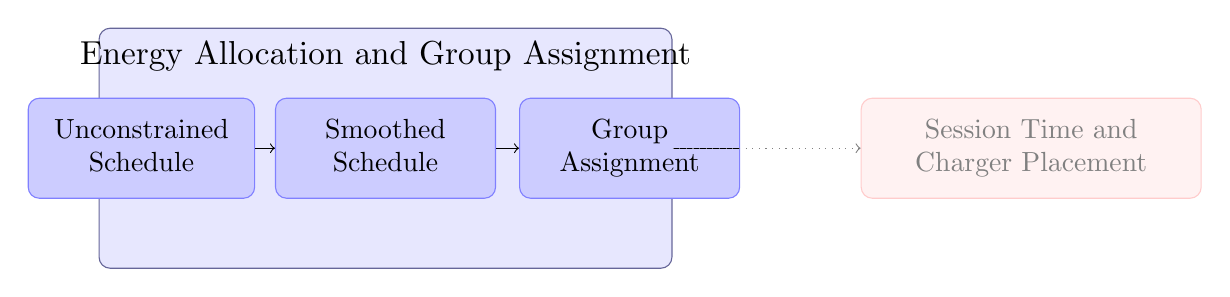
\begin{tikzpicture}
\node[rectangle, draw=gray!80!blue, fill=gray!10!blue!10, minimum width=\textwidth*0.6, minimum height=1.2in, rounded corners, label={[label distance=-0.67cm]above:\scalebox{1.2}{Energy Allocation and Group Assignment}}](outline) at (0,0){};
	\node[rectangle, draw=blue!50, fill=blue!20, minimum width=1.1in, minimum height=0.5in, rounded corners](problem1) at (-3.1,0) {\begin{tabular}{c} Unconstrained \\ Schedule\end{tabular}}; 
	\node[rectangle, draw=blue!50, fill=blue!20, minimum width=1.1in, minimum height=0.5in, rounded corners](problem2) at (0,0) {\begin{tabular}{c}Smoothed \\ Schedule\end{tabular}}; 
	\node[rectangle, draw=blue!50, fill=blue!20, minimum width=1.1in, minimum height=0.5in, rounded corners](problem3) at (3.1,0) {\begin{tabular}{c}Group \\ Assignment\end{tabular}}; 
	\node[rectangle, draw=red!20, fill=red!5, text=black!50, minimum width=1.7in, minimum height=0.5in, rounded corners](problem4) at (8.2,0){\begin{tabular}{c}Session Time and \\ Charger Placement\end{tabular}};
	\draw (problem3.east) -- (outline.east);
	\draw[->, draw=black!50, dotted] (outline.east) -- (problem4.west);
	\draw[->, draw=black] (problem1.east) -- (problem2.west);
	\draw[->, draw=black] (problem2.east) -- (problem3.west);
\end{tikzpicture}\caption{Processing chain for the energy allocation and group assignment problems} \label{fig:set1Chain}\end{figure*}

